\documentclass[a4paper,12pt]{extarticle}
\usepackage[utf8x]{inputenc}
\usepackage[T1,T2A]{fontenc}
\usepackage[russian]{babel}
\usepackage{hyperref}
\usepackage{indentfirst}
\usepackage{listings}
\usepackage{color}
\usepackage{xcolor}
\usepackage{here}
\usepackage{array}
\usepackage{multirow}
\usepackage{graphicx}
\usepackage{amsmath}

\hypersetup{
    colorlinks = false,
    linkbordercolor = {white}
}

\definecolor{string}{HTML}{B40000} % цвет строк в коде
\definecolor{comment}{HTML}{008000} % цвет комментариев в коде
\definecolor{keyword}{HTML}{1A00FF} % цвет ключевых слов в коде
\definecolor{morecomment}{HTML}{8000FF} % цвет include и других элементов в коде
\definecolor{сaptiontext}{HTML}{FFFFFF} % цвет текста заголовка в коде
\definecolor{сaptionbk}{HTML}{999999} % цвет фона заголовка в коде
\definecolor{bk}{HTML}{FFFFFF} % цвет фона в коде
\definecolor{frame}{HTML}{999999} % цвет рамки в коде
\definecolor{brackets}{HTML}{B40000} % цвет скобок в коде

\usepackage{caption}
\renewcommand{\lstlistingname}{Программа} % заголовок листингов кода

\bibliographystyle{ugost2008ls}

\usepackage{listings}
\lstset{ %
	extendedchars=\true,
	keepspaces=true,
	language=Python,						% choose the language of the code
	% Цвета
	keywordstyle=\color{keyword}\ttfamily\bfseries,
	%stringstyle=\color{string}\ttfamily,
	stringstyle=\ttfamily\color{red!50!brown},
	commentstyle=\color{comment}\ttfamily\itshape,
	morecomment=[l][\color{morecomment}]{\#},
	basicstyle=\footnotesize,		% the size of the fonts that are used for the code
	numbers=left,					% where to put the line-numbers
	numberstyle=\footnotesize,		% the size of the fonts that are used for the line-numbers
	stepnumber=1,					% the step between two line-numbers. If it is 1 each line will be numbered
	numbersep=5pt,					% how far the line-numbers are from the code
	backgroundcolor=\color{white},	% choose the background color. You must add \usepackage{color}
	showspaces=false				% show spaces adding particular underscores
	keywordstyle=color{blue}\bfseries, 
	showstringspaces=false,			% underline spaces within strings
	showtabs=false,					% show tabs within strings adding particular underscores
	frame=single,          		% adds a frame around the code
	tabsize=2,						% sets default tabsize to 2 spaces
	captionpos=t,					% sets the caption-position to top
	breaklines=true,				% sets automatic line breaking
	breakatwhitespace=false,		% sets if automatic breaks should only happen at whitespace
	escapeinside={\%*}{*)},			% if you want to add a comment within your code
	postbreak=\raisebox{0ex}[0ex][0ex]{\ensuremath{\color{red}\hookrightarrow\space}},
	texcl=true,
	inputpath=listings,                     % директория с листингами
}

\usepackage[left=2cm,right=2cm,
top=2cm,bottom=2cm,bindingoffset=0cm]{geometry}

%% Нумерация картинок по секциям
\usepackage{chngcntr}
\counterwithin{figure}{section}
\counterwithin{table}{section}

%%Точки нумерации заголовков
\usepackage{titlesec}
\titlelabel{\thetitle.\quad}
\usepackage[dotinlabels]{titletoc}

%% Оформления подписи рисунка
\addto\captionsrussian{\renewcommand{\figurename}{Рисунок}}
\captionsetup[figure]{labelsep = period}

%% Подпись таблицы
\DeclareCaptionFormat{hfillstart}{\hfill#1#2#3\par}
\captionsetup[table]{format=hfillstart,labelsep=newline,justification=centering,skip=-10pt,textfont=bf}

%% Путь к каталогу с рисунками
\graphicspath{{fig/}}

\begin{document}	% начало документа

% Титульная страница
%\begin{titlepage}	% начало титульной страницы

	\begin{center}		% выравнивание по центру

		Санкт-Петербургский Национально Исследовательский Университет\\
		информационных технологий, механики и оптики \\
		Кафедра систем управления и информатики\\[3cm]
		% название института, затем отступ 6см
		
		\huge \textbf{РЕФЕРАТ}\\[0.5cm]
		\large Электромеханические системы\\[0.1cm]
		\large Система автоматического управления квадракоптера Parrot ARDrone 2.0\\[2cm]

	\end{center}


	\begin{flushright} % выравнивание по правому краю
%		\begin{minipage}{0.5\textwidth} % врезка в половину ширины текста
%			\begin{flushleft} % выровнять её содержимое по левому краю

				\large Выполнили студенты группы P3335\\
				\large А.М. Зенкин\\[0.5cm]
				\large К.В. Карпов\\[0.5cm]
				
				\large Принял  к.т.н., доцент кафедры СУиР\\
				\sign[4cm]\large  М.С. Чежин\\
				\large Оценка: \sign\\
				«\underline{\hspace{0.7cm}}» \underline{\hspace{2cm}} \the\year г.

%			\end{flushleft}
%		\end{minipage}
	\end{flushright}
	
	\vfill % заполнить всё доступное ниже пространство

	\begin{center}
	\large Санкт-Петербург\\
	\large \the\year % вывести дату
	\end{center} % закончить выравнивание по центру

\thispagestyle{empty} % не нумеровать страницу
%\end{titlepage} % конец титульной страницы
\newpage


% Содержание
% Содержание
\renewcommand\contentsname{\centerline{Содержание}}
\tableofcontents
\thispagestyle{fancy}
\newpage




\section{Цель работы}
Ознакомление с принципами построения моделей внешних воздействий — сигналов задания и возмущений.


\section{Варианты параметров}
$\phi = 24^\circ$, $f = 2 c^{-1}$\\
		
$\Delta=	4, V=2, F=10;$\\									
\section{Ход выполнения работы}

\subsection{Исследование командного генератора гармонического сигнала}

\subsubsection{Построение математической модели:}
\begin{equation}
	\begin{split}
&\omega=2\pi f=2\cdot 3.14\cdot 2=12.56;\\
&A=\frac{\tan(\phi)}{\omega}=\frac{tan(24^\circ)}{12.56}=0.0.354;\\
&z = \begin{bmatrix}
				z_1\\
				z_2
				\end{bmatrix}, G = \begin{bmatrix}
				0 & 1\\
				-157.7536 & 0
				\end{bmatrix}, H^T = \begin{bmatrix}
				1\\
				0
				\end{bmatrix};\\
	\end{split}				
\end{equation}
				
\subsubsection{Схема моделирования командного генератора:}
\begin{figure}[H]
	\begin{center}
		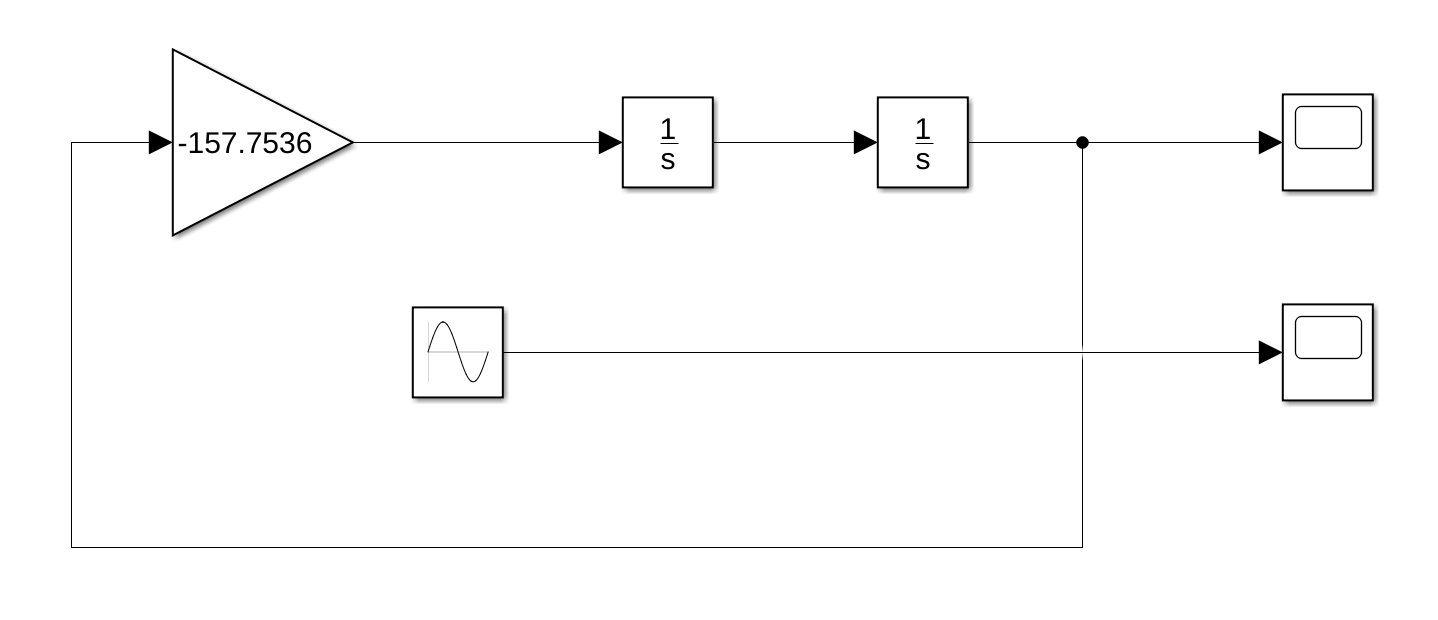
\includegraphics[scale=0.25]{s_1}
		\caption{- схема моделирования} 
		\label{pic:pic_1} % название для ссылок внутри кода
	\end{center}
\end{figure}

\subsubsection{Моделирование работы командного генератора:}
\begin{figure}[H]
	\begin{center}
		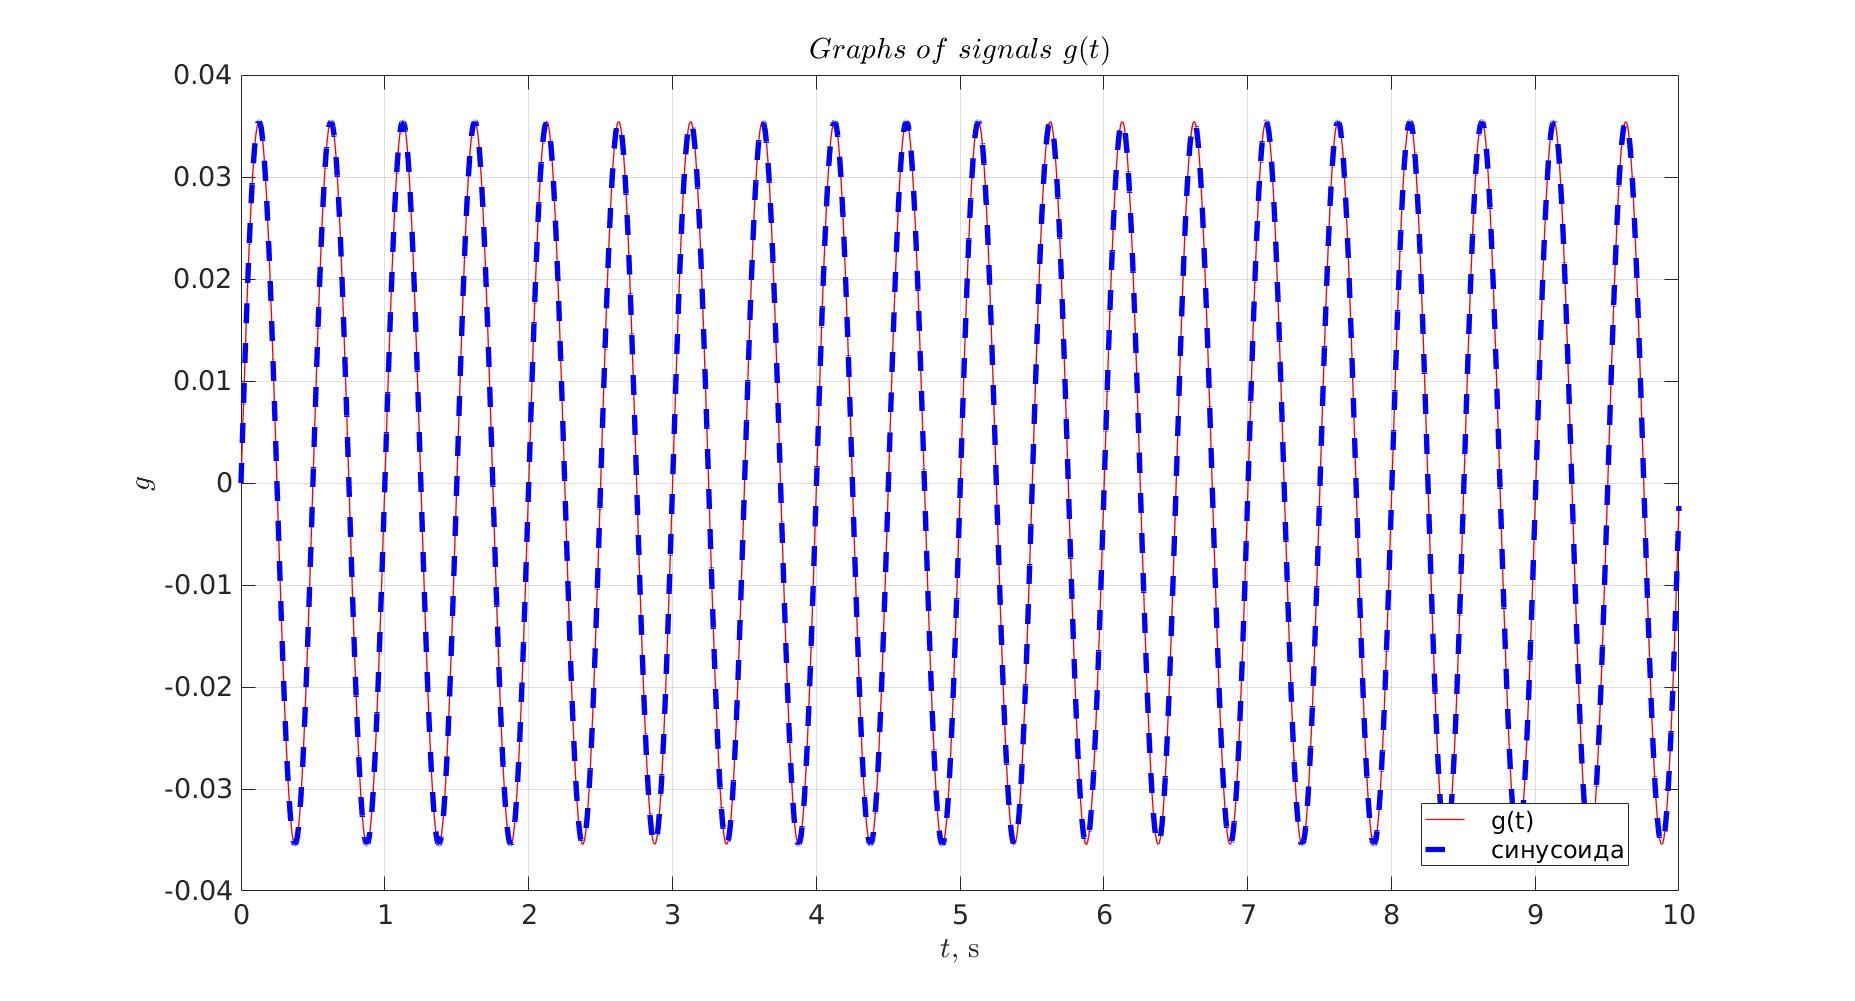
\includegraphics[scale=0.27]{g_1}
		\caption{- сигнал g(t) и синусоида} 
		\label{pic:pic_1} % название для ссылок внутри кода
	\end{center}
\end{figure}

\subsection{Исследование командного генератора сигнала с трапецеидальным графиком скорости}
\subsubsection{Построение математической модели:}
\begin{equation}
	\begin{split}
		&\Delta=	4, V=2, F=10;\\
		&t_\alpha=\left| {\dfrac{V_2-V_1}{\alpha}} \right|=\left| {\dfrac{2-0}{4}} \right|=0.5c;\\
		&t_b=\dfrac{g}{V}=\dfrac{10}{2}=5c;\\
		&t_c=\left| {\dfrac{V_2-V_1}{\alpha}} \right|=\left| {\dfrac{0-(-2)}{4}} \right|=0.5c;\\
	\end{split}				
\end{equation}

\subsubsection{Схема моделирования командного генератора:}
\begin{figure}[H]
	\begin{center}
		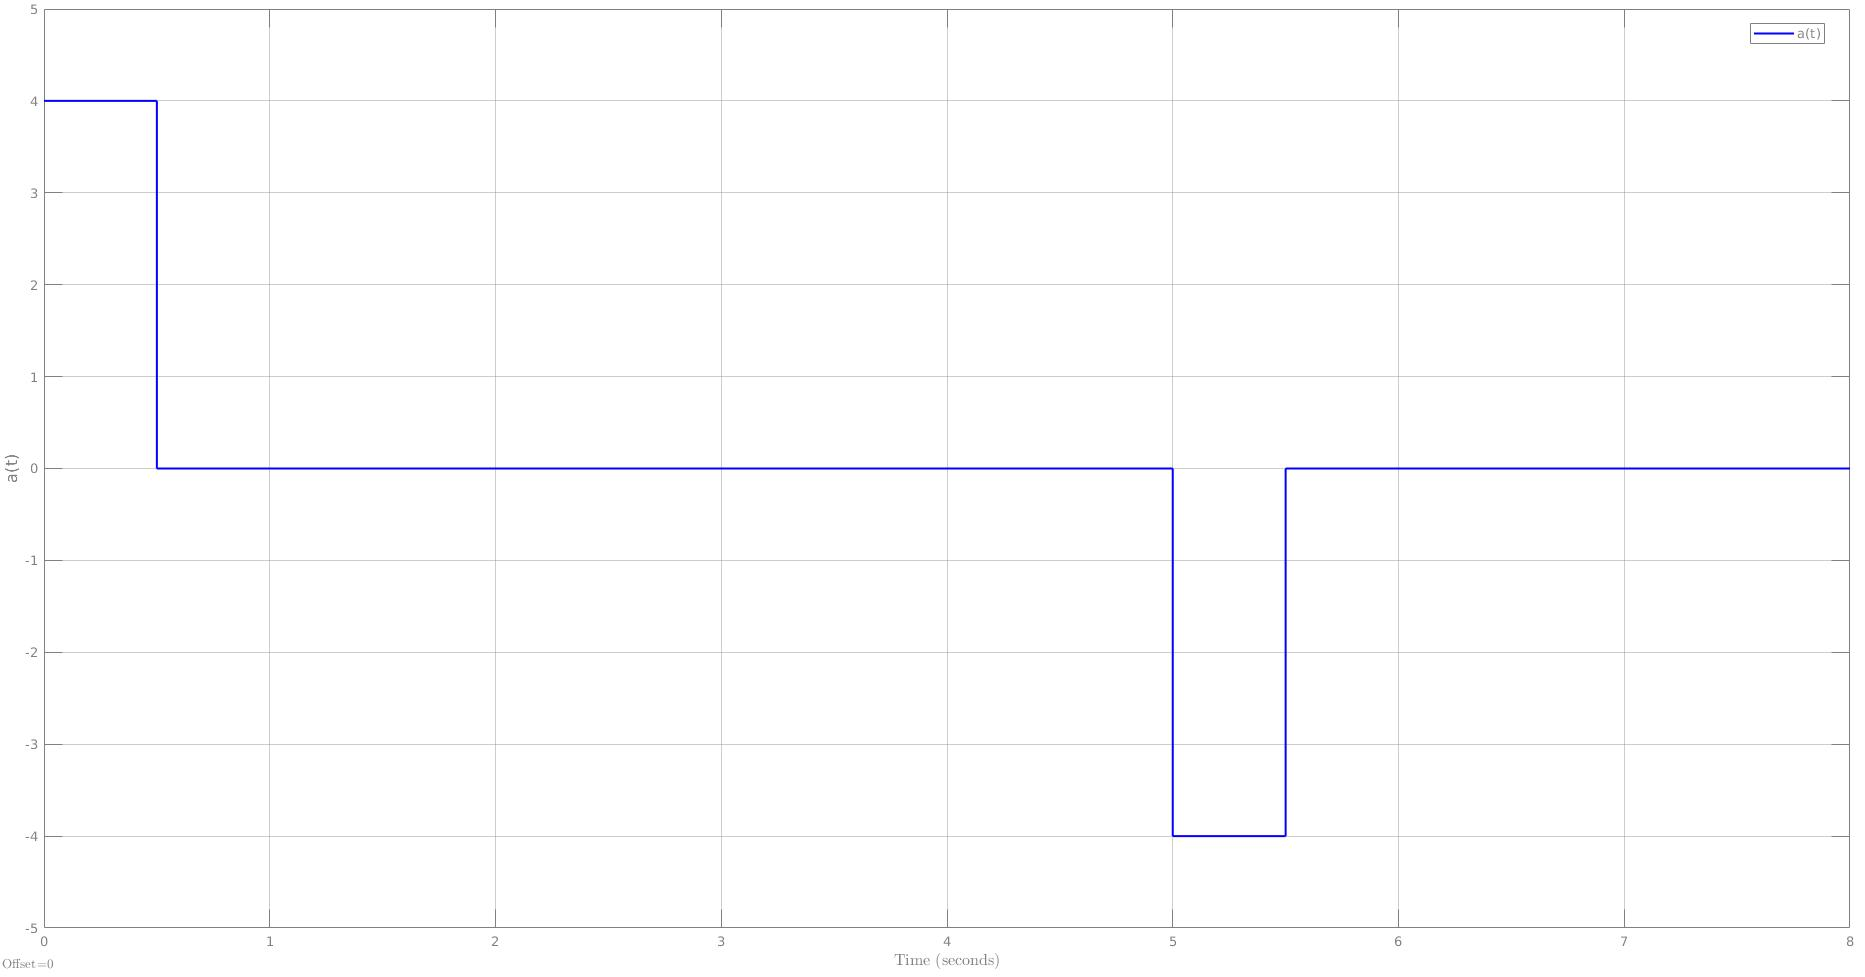
\includegraphics[scale=0.25]{g_2}
		\caption{- сигнал a(t)} 
		\label{pic:pic_1} % название для ссылок внутри кода
	\end{center}
\end{figure}

\subsubsection{Моделирование работы командного генератора:}
\begin{figure}[H]
	\begin{center}
		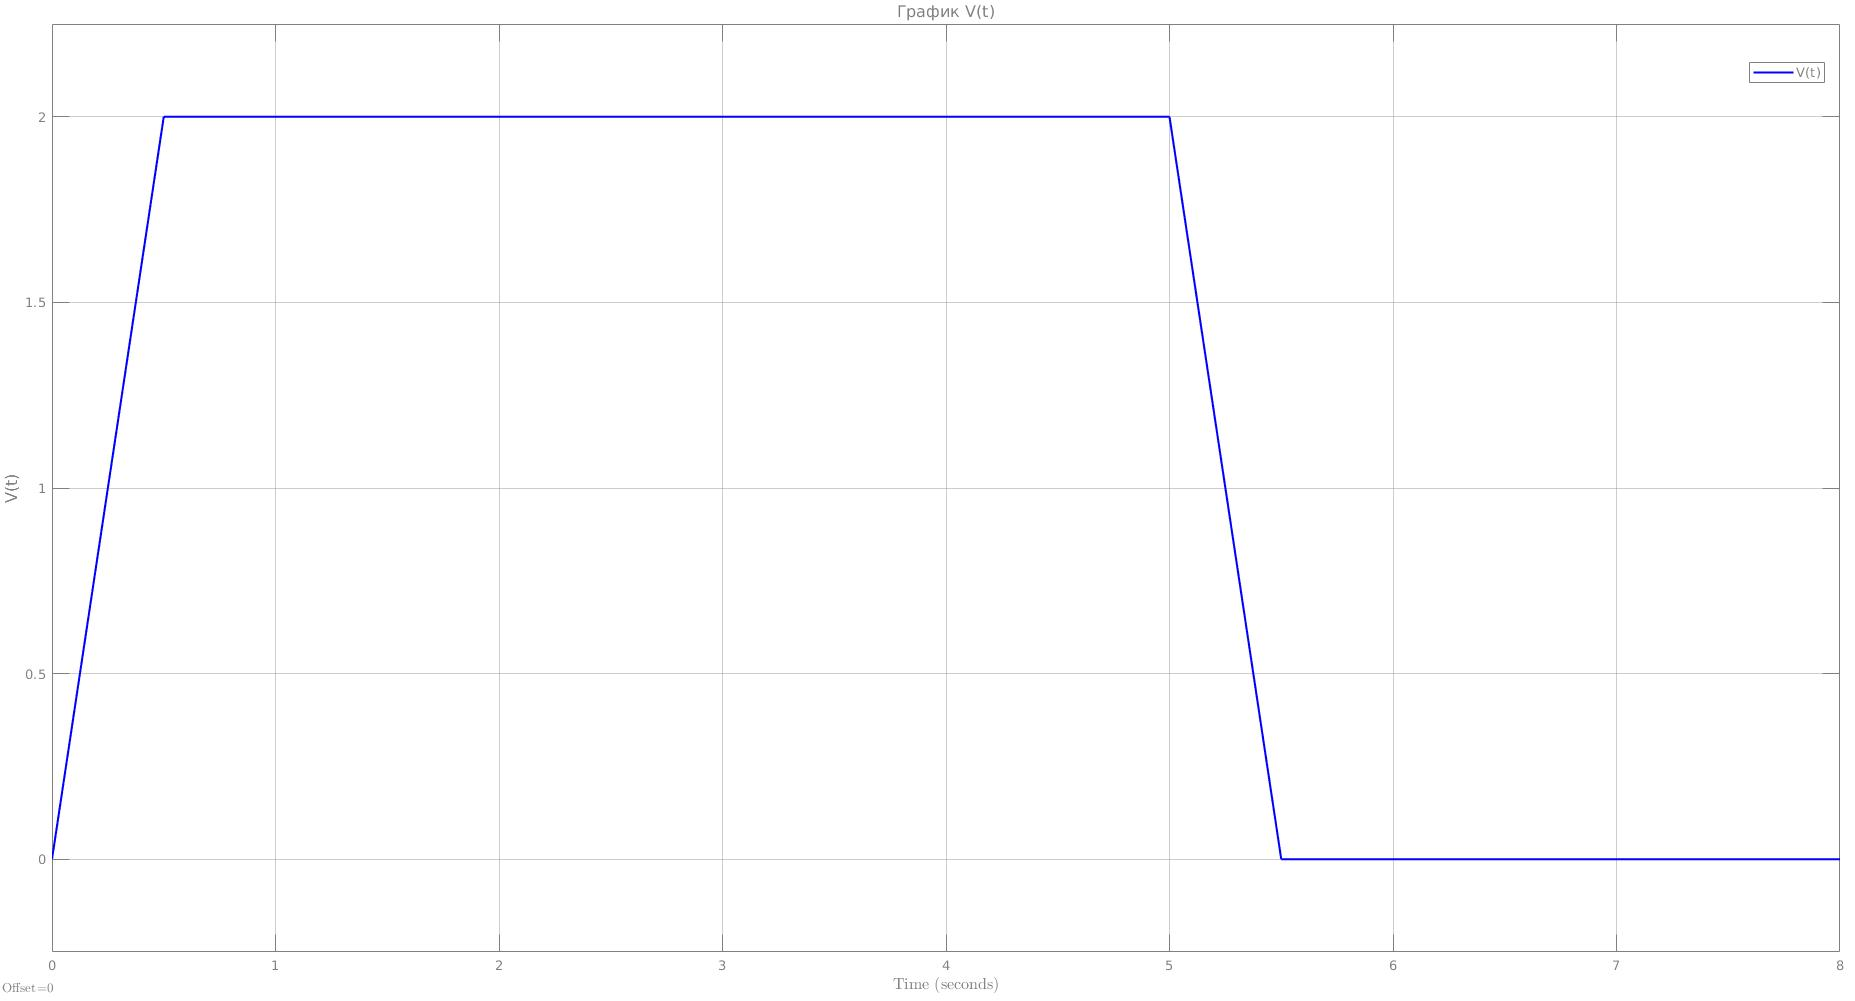
\includegraphics[scale=0.25]{g_3}
		\caption{- схема моделирования} 
		\label{pic:pic_1} % название для ссылок внутри кода
	\end{center}
\end{figure}

\begin{figure}[H]
	\begin{center}
		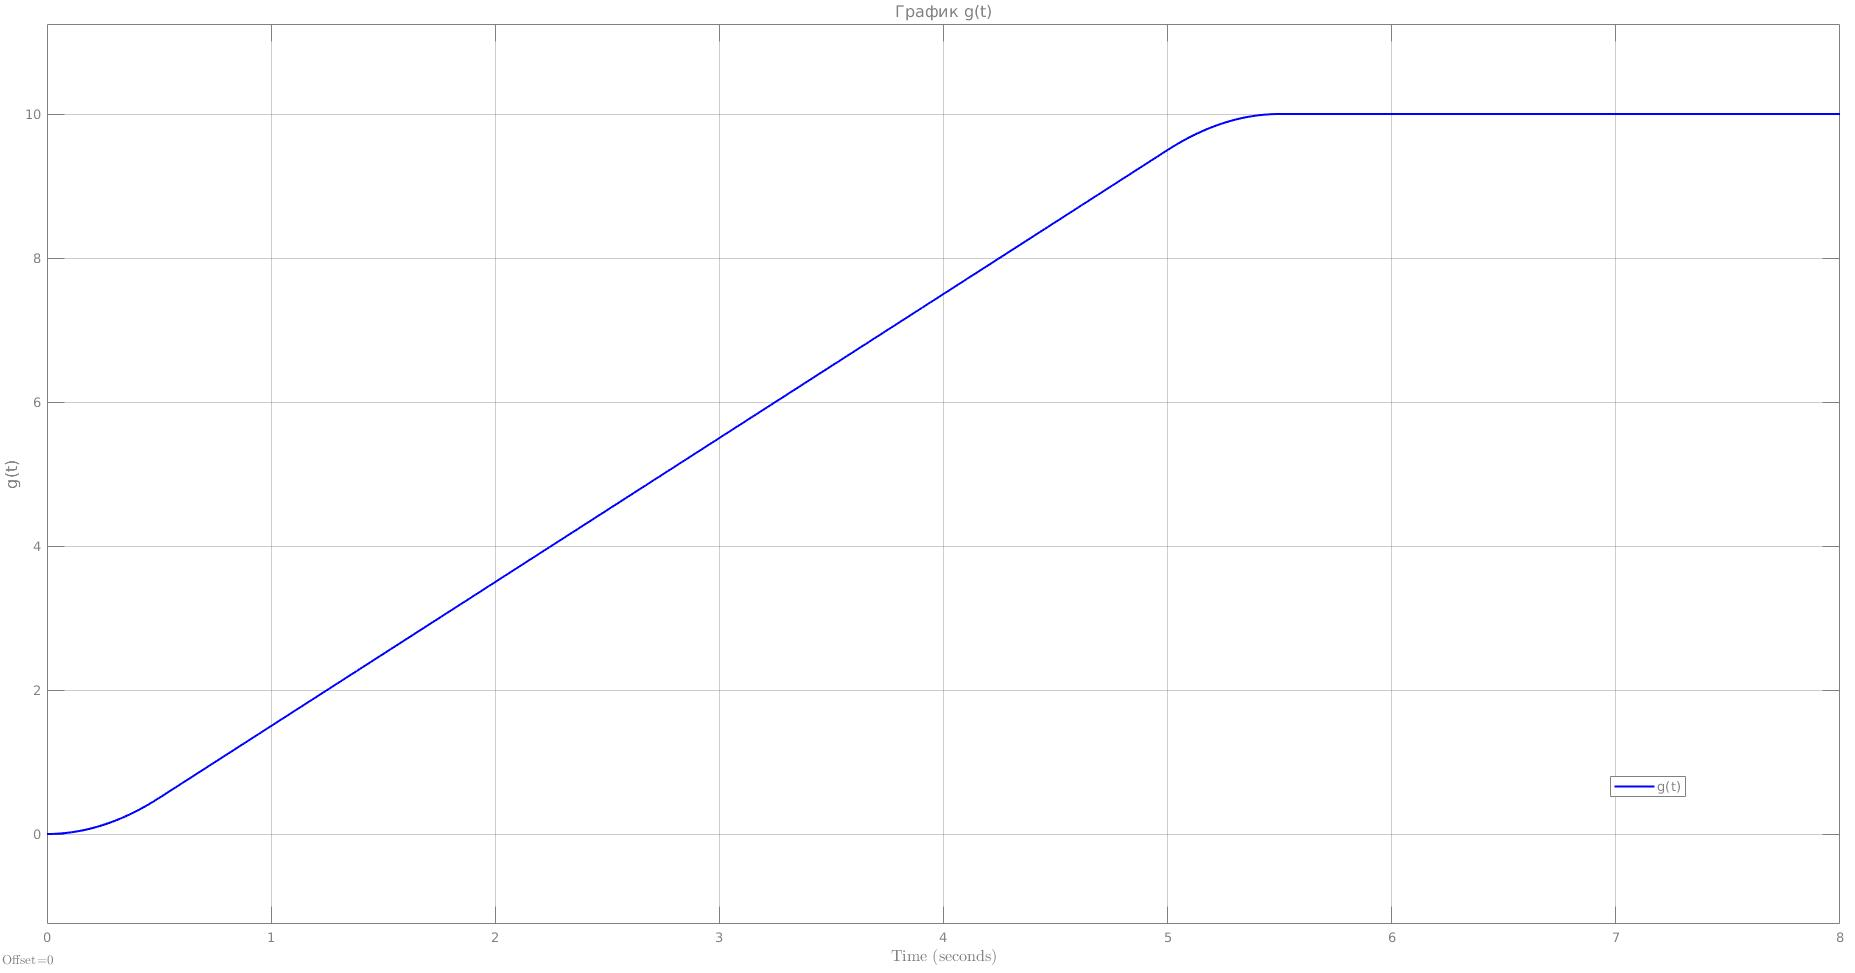
\includegraphics[scale=0.25]{g_4}
		\caption{- сигнал g(t)} 
		\label{pic:pic_1} % название для ссылок внутри кода
	\end{center}
\end{figure}

\newpage

\subsection{Исследование командного генератора возмущения}

\subsubsection{Моделирование работы командного генератора:}
\begin{figure}[H]
	\begin{center}
		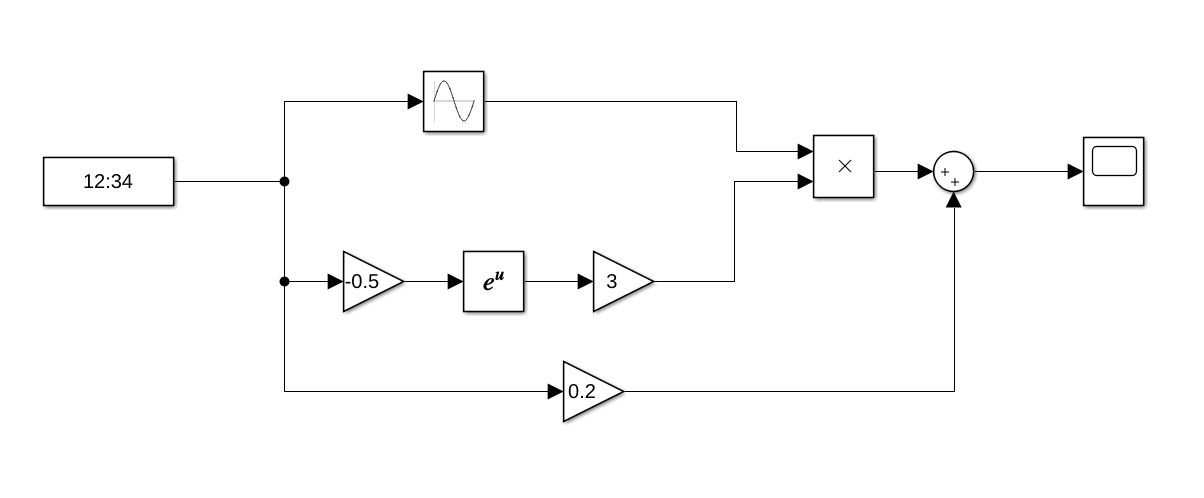
\includegraphics[scale=0.3]{s_3}
		\caption{- сигнал V(t)} 
		\label{pic:pic_1} % название для ссылок внутри кода
	\end{center}
\end{figure}

\subsubsection{Моделирование работы командного генератора:}
\begin{figure}[H]
	\begin{center}
		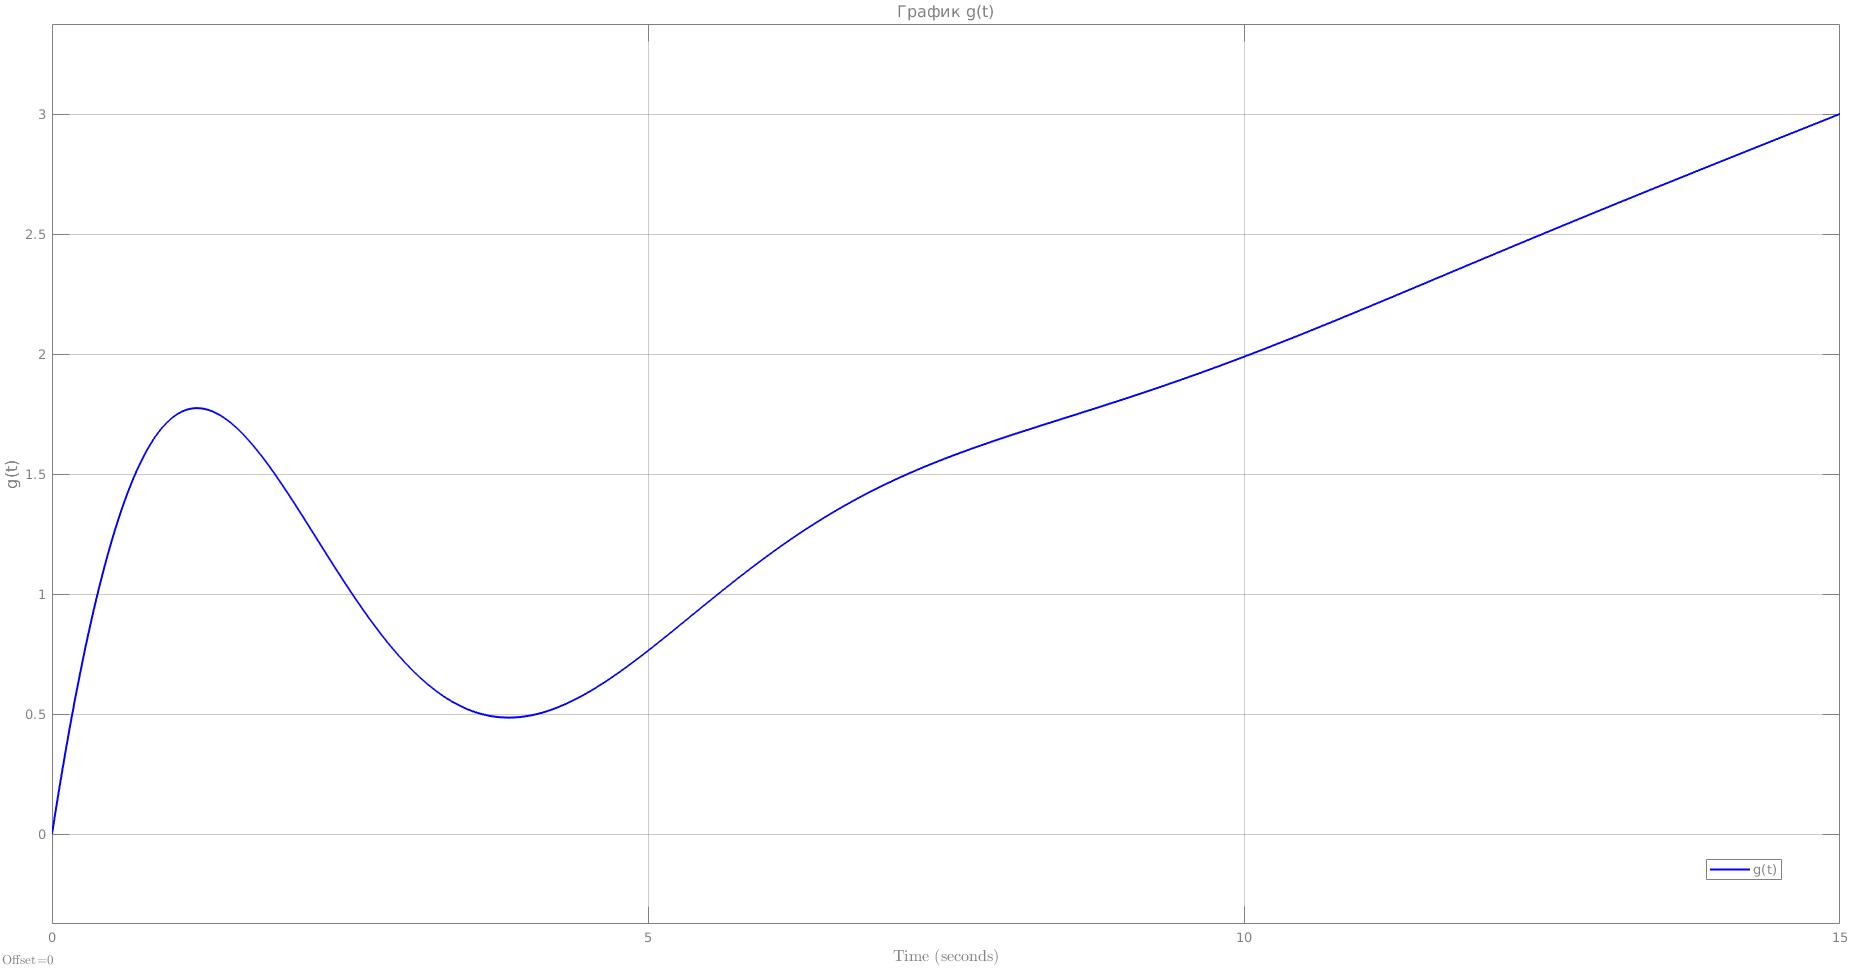
\includegraphics[scale=0.25]{g_5}
		\caption{- сигнал g(t)} 
		\label{pic:pic_1} % название для ссылок внутри кода
	\end{center}
\end{figure}

\newpage

\section{Вывод}
В данной работе было проведено ознакомление с построением моделей внешних воздействий - сигналов задания и возмущений посредствам последовательного дифференцирования, который строит дифференциальное уравнение по известному частному решению, заданному в виде функции времени.
\end{document}
